%----------------------------------------------------------------------------
\chapter{Technológia}\label{sect:technológia}
%----------------------------------------------------------------------------

+++ bevezeto a fejezethez +++

%,,,,,,,,,,,,,,,,,,,,,,,,,,,,,,,,,,,,,,,,,,,,,,,,,,,,,,,,,,,,,,,,,,,,,,,,,,,,
\section{Az OpenCV könyvtár}\label{sect:opencv}
%,,,,,,,,,,,,,,,,,,,,,,,,,,,,,,,,,,,,,,,,,,,,,,,,,,,,,,,,,,,,,,,,,,,,,,,,,,,,

Az OpenCV\footnote{\url{http://opencv.willowgarage.com/}} egy nyílt forráskódú gépi látás (computer vision) könyvtár. Elsődleges célja, keretet nyújtani \textbf{valósidejű} képfeldolgozási alkalmazások fejlesztésére. A könyvtár szabadon letölthető és felhasználható a BSD licenc\footnote{\url{http://www.linfo.org/bsdlicense.html}} keretein belül.

\bigskip

Az OpenCV projekt hivatalosan 1999-ben indult az Intel kezdeményezésében. A nagyközönségnek a 2000. évi \textit{,,IEEE Conference on Computer Vision and Pattern Recognition''} konferencián mutatkozott be, majd öt béta-verziót követően 2006-ban jutott el az 1.0-ás hivatalos kiadásig. A fejlesztése itt úgy tűnt, hogy megáll, de végül a projektet a Willow Garage\footnote{\url{http://www.willowgarage.com/}} robotikai kutatólabor 2008-ban szárnyai alá vette, és azóta is aktív fejlesztés alatt áll. 2008 októberében az 1.1-es verzióval közel egy időben látott napvilágot az elsõ hivatalos OpenCV-vel foglalkozó könyv \textit{,,Learning OpenCV: Computer Vision with the OpenCV Library''} címmel Gary Bradski és Adrian Kaehler fejlesztõk tollából \cite{opencv_book}. Az egy évvel később, 2009 októberében megjelent 2.0-ás verzióval a projekt nagy fejlődésen esett át. Ebben a verzióban található meg elõször a C++ és Python interfész (ez a meglévő C mellett már három hivatalosan fejlesztett interfészt jelent), amely az egyszerûbb kezelhetõség, új függvények mellett a meglévő eljárások teljesítmény tekintetében -- különösen többmagos rendszereken -- jobb implementációját kínálja a felhasználóknak.

\bigskip

Az OpenCV jelenlegi 2.1-es verziója elérhető FreeBSD, Linux, Mac OS és Windows operációs rendszerek alá. Széles körben, mondhatni világszerte használt, felhasználói tábora több, mint 40\,000 főt számlál. Köszönhető ez többek között annak, hogy felhasználási lehetőségei igencsak sokrétűek: több, mint 500 optimalizált algoritmust kínál annak érdekében, hogy ,,ne kelljen újra feltalálnunk a kereket''. Sebesség tekintetében érződik a kipróbált, optimalizált algoritmusok használata: az OpenCV a jelenleg elérhető leggyorsabb alternatíva gépi látás terén (\figref{opencv_speed} ábra). Teljesítménye azonban adott esetben még tovább növelhető, mivel ha Intel IPP\footnote{\url{http://software.intel.com/en-us/intel-ipp/}} (Integrated Performance Primitives) támogatást észlel, az abban található szálakra optimalizált algoritmusok használatát fogja preferálni.

\begin{figure}[!ht]
\centering
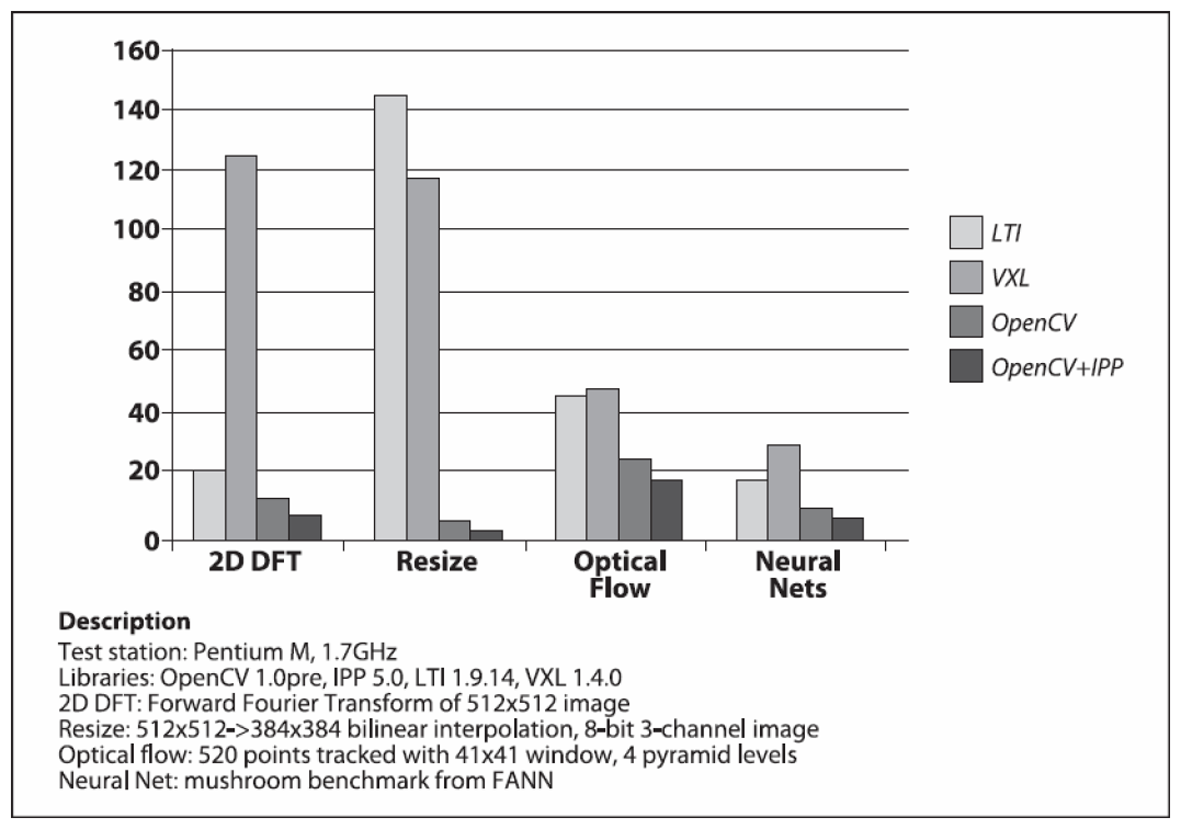
\includegraphics[width=100mm, keepaspectratio]{figures/opencv_speed.png}
\caption{Az OpenCV teljesítménye az LTI és VXL képfeldolgozási könyvtárakkal összehasonlítva.\\Forrás: \cite{opencv_book}}
\label{fig:opencv_speed}
\end{figure}

A teljes funkcionalitás részletekbe menõ bemutatása -- mint láthattuk \cite{opencv_book} -- egy könyvet is megtölt, de a teljesség igénye nélkül tekintsük át, hogy milyen alapvető jellemzői és alkalmazásai vannak a környezetnek:

\begin{itemize}

 \item alap adatstruktúrák
  \begin{itemize}
   \item mátrixok, vektorok
  \end{itemize} 

 \item mátrix és vektor manipuláció, lineáris algebra
  
 \item dinamikus adatstruktúrák
  \begin{itemize}
   \item listák, sorok, halmazok
   \item gráfok és fák
  \end{itemize}

 \item kép és videó input/output
  \begin{itemize}
   \item beolvasás fájlból (kép vagy videó) és kameráról
   \item kiírási lehetőség képként vagy videóként
  \end{itemize}

 \item előfeldolgozás
  \begin{itemize}
   \item él- és sarokkeresés
   \item mintavételezés és interpoláció
   \item színkonverzió
   \item morfológiai operátorok
  \end{itemize}

 \item struktúraanalízis
  \begin{itemize}
   \item távolság- és Hough-transzformáció
   \item kontúrfeldolgozás
   \item sablonillesztés
   \item különböző momentumok
   \item Delaunay háromszögelés
  \end{itemize}

 \item kamerakalibráció
  \begin{itemize}
   \item kalibrációs mintázatok felismerése és követése
   \item fundamentális mátrix becslés
   \item homográfia becslés
   \item sztereó megfeleltetés
  \end{itemize}
  
 \item mozgásanalízis
  \begin{itemize}
   \item optical flow
   \item mozgásszegmentálás és -követés
  \end{itemize}

 \item objektumfelismerés
  \begin{itemize}
   \item eigen-módszerek
   \item rejtett Markov-modell (Hidden Markov Model -- HMM)
  \end{itemize}
  
 \item GUI és rajzolás
  \begin{itemize}
   \item kép és videó megjelenítés
   \item billentyűzet és egérkezelés
   \item egyenes, kör, poligon, szöveg rajzolása
  \end{itemize}
  
\end{itemize}

Láthatjuk, hogy a fent felsorolt funkciókkal a gépi látás terén rengeteg egyszerűbb feladatot szinte ,,egy lépésben'', beépített, optimalizált eljárások segítségével oldhatunk meg. Ha nagyobb szabású projektbe kezdünk, akkor is hasznunkra lehet, hogy részben vagy egészében egy több tízezres felhasználói tábor (melynek jelentős részét aktív kutatók alkotják) visszajelzései alapján fejlesztett környezetre építhetjük munkánkat.

Az OpenCV számos előnye mellett hátrányként említhető meg, hogy segítségével a felhasználói felületet csak nagyon leegyszerűsített módon szabhatjuk testre. Igaz, hogy a könyvtár feladata elsősorban a képfeldolgozás és nem a megjelenítés, így ebből a nézőpontból a beépített kép és videó megjelenítési lehetőség, billentyűzet- és egérkezelés valamint trackbarok (csúsztatható kezelőszerv értékek beállítására) létrehozásának lehetősége inkább hozzáadott értékként jelenik meg. Azonban ez nem változtat azon a tényen, hogy ha igény van felhasználóbarát kezelőfelület készítésére, az OpenCV-t integrálnunk kell valamely elterjedt grafikus felhasználói felület toolkittel.

\bigskip

+++ uj funkciok, Qt felulet, atnezni +++

%,,,,,,,,,,,,,,,,,,,,,,,,,,,,,,,,,,,,,,,,,,,,,,,,,,,,,,,,,,,,,,,,,,,,,,,,,,,,
\section{A Qt keretrendszer}\label{sect:qt}
%,,,,,,,,,,,,,,,,,,,,,,,,,,,,,,,,,,,,,,,,,,,,,,,,,,,,,,,,,,,,,,,,,,,,,,,,,,,,

+++ Qt-rol osszefoglalo, Qt creator, screenshot, nyelvek +++

%,,,,,,,,,,,,,,,,,,,,,,,,,,,,,,,,,,,,,,,,,,,,,,,,,,,,,,,,,,,,,,,,,,,,,,,,,,,,
\section{Módosított kamera}\label{sect:infracam}
%,,,,,,,,,,,,,,,,,,,,,,,,,,,,,,,,,,,,,,,,,,,,,,,,,,,,,,,,,,,,,,,,,,,,,,,,,,,,

+++ kamera infok, LED csere, fenykep +++